% Copyright (c)  2005-2010 EDF-EADS-PHIMECA.
% Permission is granted to copy, distribute and/or modify this document
% under the terms of the GNU Free Documentation License, Version 1.2
% or any later version published by the Free Software Foundation;
% with no Invariant Sections, no Front-Cover Texts, and no Back-Cover
% Texts.  A copy of the license is included in the section entitled "GNU
% Free Documentation License".
\renewcommand{\etapemethodo}{B}
\renewcommand{\nomfichier}{docref_B11_KernelSmoothing}
\renewcommand{\titrefiche}{Kernel Smoothing}

\Header

\MathematicalDescription{

  Kernel smoothing is a non parametric estimation method of the probability density function of a distribution. \\
  In dimension 1, the kernel smoothed probability density function $\hat{p}$ has the following expression, where $K$ is the univariate kernel, $n$ the numerical sample size and $(X_1, \cdots, X_n) \in \mathbb{R}^n$ the univariate random sample with $\forall i, \, \, X_i \in \mathbb{R}$ :
  \begin{equation}
    \label{kernelSmooth}
    \hat{p}(x) = \displaystyle \frac{1}{nh}\sum_{i=1}^{n} K\left(\frac{x-X_i}{h}\right)
  \end{equation}
  The kernel $K$ is a function satisfying $\int K(x)\, dx=1$. Usually, $K$ is chosen to be a unimodal probability density fucntion that is symmetric about 0.\\
  The parameter $h$ is called the \emph{bandwidth}.\\


  In dimension $d>1$, the kernel may be defined as a product kernel $K_d$, as follows where $\vect{x} = (x_1, \cdots, x_d)\in \mathbb{R}^d$  :
  $$
  K_d(\vect{x}) = \displaystyle \prod_{j=1}^{j=d} K(x_j)
  $$
  which leads to the kernel smoothed probability density function in dimension $d$, where $(\vect{X}_1, \cdots, \vect{X}_n)$ is the d-variate random  sample which components are denoted $\vect{X}_i = (X_{i1}, \dots, X_{id})$ :
  $$
  \hat{p}(\vect{x}) = \displaystyle \frac{1}{N \prod_{j=1}^{j=d}h_j} \sum_{i=1}^{N} K_d\left(\frac{x_1 - X_{i1} }{h_1}, \dots, \frac{x_d - X_{id}}{h_d}\right)
  $$
  Let's note that the bandwidth is the vector $\vect{h} = (h_1, \cdots, h_d)$. \\

  The quality of the approximation may be controlled by the AMISE (Asymptotic Mean Integrated Square error) criteria defined as :
  $$
  \left\{
    \begin{array}{lcl}
      AMISE(\hat{p}) & = & \mbox{two first terms in the series expansion with respect to $n$ in } MISE(\hat{p}) \\
      MISE(\hat{p}) & = & \mathbb{E}_\vect{X}[||\hat{p} - p||^2_{L_2}]   =  \int \, MSE(\hat{p}, \vect{x}) \, d\vect{x}  \\
      MSE(\hat{p}, \vect{x})&  =  & \left[ \mathbb{E}_\vect{X}[\hat{p}(\vect{x})] - p(\vect{x})\right]^2 + Var_\vect{X}(\hat{p}(\vect{x}))
    \end{array}
  \right.
  $$


  The quality of the estimation essentially depends on the value of the bandwidth $h$. The bandwidth that minimizes the AMISE criteria  has the expression (given in dimension 1) :
  \begin{equation}
    \label{AMISE1}
    h_{AMISE}(K) = \displaystyle \left[ \frac{R(K)}{\mu_2(K)^2R(p^{(2)})}\right]^{\frac{1}{5}}n^{-\frac{1}{5}}
  \end{equation}
  where  $R(K) = \int K(\vect{x})^2\, d\vect{x}$ and $\mu_2(K) = \int \vect{x}^2K(\vect{x})\, d\vect{x} = \sigma_K^2$.\\
  If we note that $R(p^{(r)}) = (-1)^r\Phi_{2r}$ with $\Phi_r = \int p^{(r)}p(x)\, dx = \mathbb{E}_\vect{X}[p^{(r)}]$, then relation (\ref{AMISE1}) writes :
  \begin{equation}
    \label{AMISE}
    h_{AMISE}(K) = \displaystyle \left[ \frac{R(K)}{\mu_2(K)^2\Phi_4}\right]^{\frac{1}{5}}n^{-\frac{1}{5}}
  \end{equation}

  Several rules exist to  evaluate the optimal bandwidth $ h_{AMISE}(K)$ : all efforts are concentrated on the evaluation of the term $\Phi_4$. We give here the most usual rules :
  \begin{itemize}
  \item the \emph{Silverman rule} in dimension 1,
  \item the plug-in bandwidth selection - \emph{Solve-the-equation} method in dimension $d$,
  \item the \emph{Scott rule} in dimension d.
  \end{itemize}



  \vspace*{0.5cm}
  \textbf{Silverman rule (dimension 1)}\\

  In the case where the density $p$ is normal with standard deviation $\sigma$, then the term $\Phi_4$ can be exactly evaluated. In that particular case,  the optimal bandwidth of relation (\ref{AMISE}) with respect to the AMISE criteria writes as follows :
  \begin{equation}
    \label{pNormal}
    h^{p = normal}_{AMISE}(K) = \displaystyle \left[ \frac{8\sqrt{\pi} R(K)}{3\mu_2(K)^2}\right]^{\frac{1}{5}}\sigma n^{-\frac{1}{5}}
  \end{equation}

  An estimator of $h^{p= normal}_{AMISE}(K)$ is obtained by replacing $\sigma$ by its estimator $\hat{\sigma}^n$,  evaluated from the  numerical sample $(X_1, \dots, X_n)$ :
  \begin{equation}
    \label{Estimpnormal}
    \hat{h}^{p = normal}_{AMISE}(K) = \displaystyle \left[ \frac{8\sqrt{\pi} R(K)}{3\mu_2(K)^2}\right]^{\frac{1}{5}}\hat{\sigma}^n n^{-\frac{1}{5}}
  \end{equation}

  The Silverman rule consists in considering $\hat{h}^{p = normal}_{AMISE}(K)$ of relation (\ref{Estimpnormal}) even if the density $p$ is not normal :
  \begin{equation}
    \label{Silverman}
    h^{Silver}(K) = \displaystyle \left[ \frac{8\sqrt{\pi} R(K)}{3\mu_2(K)^2}\right]^{\frac{1}{5}}\hat{\sigma}^n n^{-\frac{1}{5}}
  \end{equation}

  Relation (\ref{Silverman}) is empirical and gives good results when the density is not \emph{far} from a normal one.




  \vspace*{0.5cm}

  \textbf{Plug-in bandwidth selection - \emph{Solve-the-equation} method (dimension 1)}\\



  Relation (\ref{AMISE}) requires the evaluation of the quantity $\Phi_4$. As a generale rule, we use the estimator $\hat{\Phi}_r$ of $\Phi_r$ defined by :
  \begin{equation}
    \label{EstimPhir}
    \hat{\Phi}_r = \displaystyle \frac{1}{n}\sum_{i=1}^{n} \hat{p}^{(r)}(X_i)
  \end{equation}

  Derivating relation (\ref{kernelSmooth}) leads to :
  \begin{equation}
    \label{kernelSmoothDerivative}
    \hat{p}^{(r)}(x) = \displaystyle \frac{1}{nh^{r+1}}\sum_{i=1}^{n} K^{(r)}\left(\frac{x-X_i}{h}\right)
  \end{equation}
  and then the estimator $\hat{\Phi}_r(h)$ is defined as :
  \begin{equation}
    \label{EstimPhirFin}
    \hat{\Phi}_r(h) = \displaystyle \frac{1}{n^2h^{r+1}}\sum_{i=1}^{n}\sum_{j=1}^{n} K^{(r)}\left(\frac{X_i-X_j}{h}\right)
  \end{equation}
  We note that   $\hat{\Phi}_r(h)$ depends of the parameter $h$ which can be taken in order to minimize the AMSE (Asymptotic Mean  Square Error) criteria evaluated between $\Phi_r$ and  $\hat{\Phi}_r(h)$. The optimal parameter $h$ is :
  \begin{equation}
    \label{optimHamse}
    h^{(r)}_{AMSE} = \displaystyle \left(\frac{-2K^{(r)}(0)}{\mu_2(K)\Phi_{r+2}}\right)^{\frac{1}{r+3}}n^{-\frac{1}{r+3}}
  \end{equation}





  Given that preliminary results, the solve-the-equation plug-in method  proceeds as follows :
  \begin{enumerate}
  \item Relation (\ref{AMISE}) defines $h_{AMISE}(K)$ as a function of $\Phi_4$ we denote here as :
    \begin{equation}
      \label{rel1}
      h_{AMISE}(K) = t(\Phi_4)
    \end{equation}
  \item The term  $\Phi_4$ is approximated by its estimator defined in (\ref{EstimPhirFin}) evaluated with its optimal parameter $h^{(4)}_{AMSE}$ defined in (\ref{optimHamse}) :
    \begin{equation}
      \label{h4}
      h^{(4)}_{AMSE} = \displaystyle \left(\frac{-2K^{(4)}(0)}{\mu_2(K)\Phi_{6}}\right)^{\frac{1}{7}}n^{-\frac{1}{7}}
    \end{equation}
    which leads to a relation of type :
    \begin{equation}
      \label{rel2}
      \Phi_4 \simeq  \hat{\Phi}_4(h^{(4)}_{AMSE})
    \end{equation}

  \item Relations (\ref{AMISE}) and (\ref{h4}) lead to the new one :
    \begin{equation}
      \label{h4hAmise}
      h^{(4)}_{AMSE} = \displaystyle \left( \frac{-2K^{(4)}(0)\mu_2(K)\Phi_4}{R(K)\Phi_{6}}\right) ^{\frac{1}{7}}h_{AMISE}(K)^{\frac{5}{7}}
    \end{equation}

    which rewrites :
    \begin{equation}
      \label{rel3}
      h^{(4)}_{AMSE} = l(h_{AMISE}(K))
    \end{equation}

  \item Relation (\ref{h4hAmise}) depends on both terms $\Phi_4$ and $\Phi_6$ which are evaluated with their estimators defined in (\ref{EstimPhirFin}) respectively with their AMSE optimal parameters $g_1$ and $g_2$ (see relation (\ref{optimHamse})).  It leads to the expressions~:
    \begin{equation}
      \label{g12}
      \left\{
        \begin{array}{lcl}
          g_1 & = & \displaystyle \left(\frac{-2K^{(4)}(0)}{\mu_2(K)\Phi_{6}}\right)^{\frac{1}{7}}n^{-\frac{1}{7}}\\
          g_2 & = & \displaystyle \left(\frac{-2K^{(6)}(0)}{\mu_2(K)\Phi_{8}}\right)^{\frac{1}{7}}n^{-\frac{1}{9}}
        \end{array}
      \right.
    \end{equation}

  \item In order to evaluate $\Phi_6$ and $\Phi_8$, we suppose that the density $p$ is normal with a variance $\sigma^2$ which is approximated by the empirical variance of the numerical sample, which leads to :
    \begin{equation}
      \label{Phi68}
      \left\{
        \begin{array}{lcl}
          \hat{\Phi}_6 & = & \displaystyle \frac{-15}{16\sqrt{\pi}}\hat{\sigma}^{-7}\\
          \hat{\Phi}_8 & = & \displaystyle \frac{105^{\strut}}{32\sqrt{\pi}}\hat{\sigma}^{-9}
        \end{array}
      \right.
    \end{equation}
  \end{enumerate}

  Then, to resume, thanks to relations (\ref{rel1}), (\ref{rel2}), (\ref{rel3}), (\ref{g12}) and (\ref{Phi68}), the optimal bandwidth is solution of the equation :
  \begin{equation}
    \label{equhAmise}
    \boldsymbol{h_{AMISE}(K) = t \circ \hat{\Phi}_4 \circ l (h_{AMISE}(K))}
  \end{equation}





  \vspace*{0.5cm}


  \textbf{Scott rule (dimension d)}\\

  The Scott rule is a simplification of the Silverman rule generalized to the dimension $d$ which is optimal when the density $p$ is normal with independent components. In all the other cases, it gives an empirical rule that gives good result when the density $p$ is not \emph{far} from the normal one. For examples, the Scott bandwidth may appear too large when $p$ presents several maximum.\\

  The Silverman rule given in dimension 1 in relation (\ref{Silverman}) can be generalized in dimension $d$ as follows : if we suppose  that the density $p$ is normal with independent components, in dimension $d$ and that we use the normal kernel $N(0,1)$ to estimate it, then the optimal bandwidth vector $\vect{h}$ with respect to the AMISE criteria writes as follows :
  \begin{equation}
    \label{SilvermanNormalKernel}
    \vect{h}^{Silver}(N) = \left(\left(\frac{4}{d+2}\right)^{1/(d+4)}\hat{\sigma}_i^n n^{-1/(d+4)}\right)_i
  \end{equation}
  where $\hat{\sigma}_i^n$ is the standard deviation of the $i-th$ component of the sample $(\vect{X}_1, \cdots, \vect{X}_n)$, and $\sigma_K$ the standard deviation of the 1D kernel $K$.\\



  The Scott proposition is  a simplification of the Silverman rule, based on the fact that the coefficient $\left(\frac{4}{d+2}\right)^{1/(d+4)}$ remains in $[0.924, 1.059]$ when the dimension $d$ varies. Thus, Scott fixed it to $1$ :
  \begin{equation}
    \label{coefficientScott}
    \left(\frac{4}{d+2}\right)^{1/(d+4)} \simeq 1
  \end{equation}
  which leads to the simplified expression :
  \begin{equation}
    \label{SilvermanNormalKernelSimplif}
    \vect{h}^{Silver}(N) \simeq \left( \hat{\sigma}_i^n n^{-1/(d+4)}\right)_i
  \end{equation}




  Furthermore, in the general case, we have from relation (\ref{AMISE1}) :
  \begin{equation}
    \label{ChangeBandwidth}
    \frac{h_{AMISE}(K_1)}{h_{AMISE}(K_2)}=\frac{\sigma_{K_2}}{\sigma_{K_1}}\left[\frac{\sigma_{K_1}R(K_1)}{\sigma_{K_2}R(K_2)}\right]^{1/5}
  \end{equation}

  Considering that $\sigma_{K}R(K) \simeq 1$ whatever the kernel $K$,   relation (\ref{ChangeBandwidth}) simplifies in :
  \begin{equation}
    \label{SimplifiedChangeBandwidth}
    h_{AMISE}(K_1) \simeq h_{AMISE}(K_2)\frac{\sigma_{K_2}}{\sigma_{K_1}}
  \end{equation}





  If we consider the normal kernel $N(0,1)$ for $K_2$, then relation (\ref{SimplifiedChangeBandwidth}) writes in a more general notation :
  \begin{equation}
    \label{SimplifiedChangeBandwidthNormal}
    h_{AMISE}(K) \simeq h_{AMISE}(N)\frac{1}{\sigma_{K}}
  \end{equation}

  If $h_{AMISE}(N)$ is evaluated with the Silverman rule, (\ref{SimplifiedChangeBandwidthNormal}) rewrites :
  \begin{equation}
    \label{SimplifiedChangeBandwidthSilvNormal}
    h^{Silver}(K) \simeq h^{Silver}(N)\frac{1}{\sigma_{K}}
  \end{equation}



  At last, from relation (\ref{SilvermanNormalKernelSimplif}) and (\ref{SimplifiedChangeBandwidthSilvNormal}) applied in each direction $i$, we deduce the Scott rule :
  \begin{equation}
    \label{ScottRule}
    \boldsymbol{\vect{h}^{Scott} = \left(\frac{\hat{\sigma}_i^n}{\sigma_K}n^{-1/(d+4)}\right)_i}
  \end{equation}




  \vspace*{0.5cm}

  \textbf{Boundary treatment}\\


  In dimension 1, the boundary effects may be taken into account in Open TURNS : the boundaries are automatically detected from the numerical sample (with the $min$ and $max$ functions) and the kernel smoothed PDF is corrected in the boundary areas to remain within the boundaries, according to the miroring technique :
  \begin{itemize}
  \item the Scott bandwidth is evaluated from the numerical sample : $h$
  \item two subsamples are extracted from the inital numerical sample, containing all the points within the range $[min, min + h[$ and  $]max-h, max]$,
  \item both subsamples are transformed into their symmetric samples with respect their respective boundary : its results two samples within the range  $]min-h, min]$ and  $[max, max+h[$,
  \item a kernel smoothed PDF is built from the new numerical sample composed with the initial one and the two new ones, with the previous bandwidth $h$,
  \item this last kernel smoothed PDF is truncated within the inital range  $[min, max]$ (conditionnal PDF).
  \end{itemize}



  \vspace*{0.5cm}

  \textbf{Implementation in Open TURNS}\\
  The choice of the kind of the kernel is free in Open TURNS : it is possible to select any 1D distribution and to define it as a kernel. However, in order to optimize the efficiency of the kernel smoothing fitting (it means to minimise the AMISE error), it is recommended to select a {\bf symmetric distribution} for the kernel. \\
  All the distribution default constructors of Open TURNS create a symmetric default distribution when possible. It is also possible to work with the Epanechnikov kernel, which is a $Beta(r=2, t=4, a=-1, b=1)$. \\
  The default kernel is a product of standard Normal distribution. The dimension of the product is automatically evaluated from the random sample.\\

  The bandwidth $\vect{h}$ may be fixed by the User. However, it is recommended to let Open TURNS evaluate it automatically from the numerical sample according to the following rules :\\

  {\bf In dimension $d$}, Open TURNS automatically applies the Scott rule.\\




  {\bf In dimension 1}, the automatic bandwidth selection method depends  on the size $n$ of the numerical sample. As a matter of fact, the computation bottleneck is the estimation of the estimators $\hat{\Phi}_r$ as it requires the evaluation of a double summation on the numerical sample, which has a cost of $\mathcal{O}(n^2)$.
  \begin{itemize}
  \item if $n \leq 250$, the Solve-the-equation  plug-in method is used on the entire numerical sample. The optimal bandwidth $h_{AMISE}(N)$  is first evaluated when considering a normal kernel, resolving equation (\ref{equhAmise}) for the Normal kernel. Then relation (\ref{SimplifiedChangeBandwidthNormal}) is applied in order to evaluate $h_{AMISE}(K)$.

  \item if $n>250$, the Solve-the-equation  plug-in method is too computationnally expensive. Then, Open TURNS proceeds as follows :
    \begin{enumerate}
    \item Open TURNS evaluates the bandwidth $h^{n_1, PI}_{AMISE}(N)$ with the plug-in method applied on the first $n_1 = 250$ points of the numerical sample, using the Normal kernel $N$ (by solving equation (\ref{equhAmise}) with $K=N$);
    \item Open TURNS evaluates the bandwidth $h^{n_1, Silver}(N)$ with the Silverman rule applied on the first $n_1 = 250$ points of the numerical sample, using the Normal kernel $N$ (relation (\ref{Silverman}) with $K=N$);
    \item Open TURNS evaluates the bandwidth $h^{n, Silver}(N)$ with the Silverman rule applied on the entire numerical sample, using the Normal kernel $N$ (relation (\ref{Silverman}) with $K=N$);
    \item Considering from relation (\ref{AMISE})  that :
      \begin{equation}
        \label{fracSilvAmise}
        \displaystyle \frac{h^{Silver}(K)}{h_{AMISE}(K)} = \left[ \frac{\Phi_4(p=normal)}{\Phi_4(p)}\right]^{\frac{1}{5}}
      \end{equation}
      which is independent of the size $n$, we have the final relation :
      \begin{equation}
        \label{fracSilvAmiseFin}
        \displaystyle h^{n, PI}_{AMISE}(N) = \frac{h^{n_1, PI}_{AMISE}(N)}{h^{n_1, Silver}(N)}h^{n, Silver}(N)
      \end{equation}
      Then, if the User has chosen the kernel $K$ rather than the normal  kernel $N$, relation (\ref{SimplifiedChangeBandwidthNormal}) is used, which leads to :
      \begin{equation}
        \label{OTrule}
        \displaystyle h^{n, PI}_{AMISE}(K) = \frac{1}{\sigma_K} \frac{h^{n_1, PI}_{AMISE}(N)}{h^{n_1, Silver}_{AMISE}(N)}h^{n, Silver}_{AMISE}(N)
      \end{equation}
    \end{enumerate}
  \end{itemize}





}
{
  -
}

\Methodology{
  This kernel smoothing method can be used to estimate the probability density function :
  \begin{itemize}
  \item of the distribution of the input random variable (Step B of the global methodology),
  \item of the distribution of the ouput variable of interest (Step C of the global methodology).
  \end{itemize}


}
{


  The following references gives details on the method :
  \begin{itemize}
  \item \emph{Kernel smoothing}, M.P. Wand and M.C. Jones, Chapman \& Hall/CRC edition, ISNB 0-412-55270-1.
  \item \emph{Multivariate Density Estimation, practice and Visualisation, Theory}, David W. Scott, Wiley edition.
  \end{itemize}



}

\Example{

  \textbf{Choice of the bandwidth $h$}\\

  This example illustrates the effect of the choice of the bandwidth $h$ on the estimation of the pdf compared to the optimal one. Depending on the choice of $h$, one could observe for the same size $N$ of input values over-smoothing effects or under-smoothing effects. \\

  \textbf{\textit{Oversmoothing effect}}\\
  In this case, $h$ is bigger than the optimal choice $h_{opt}$. The effect of the values is more widely spread as in the optimal case.

  \begin{center}
    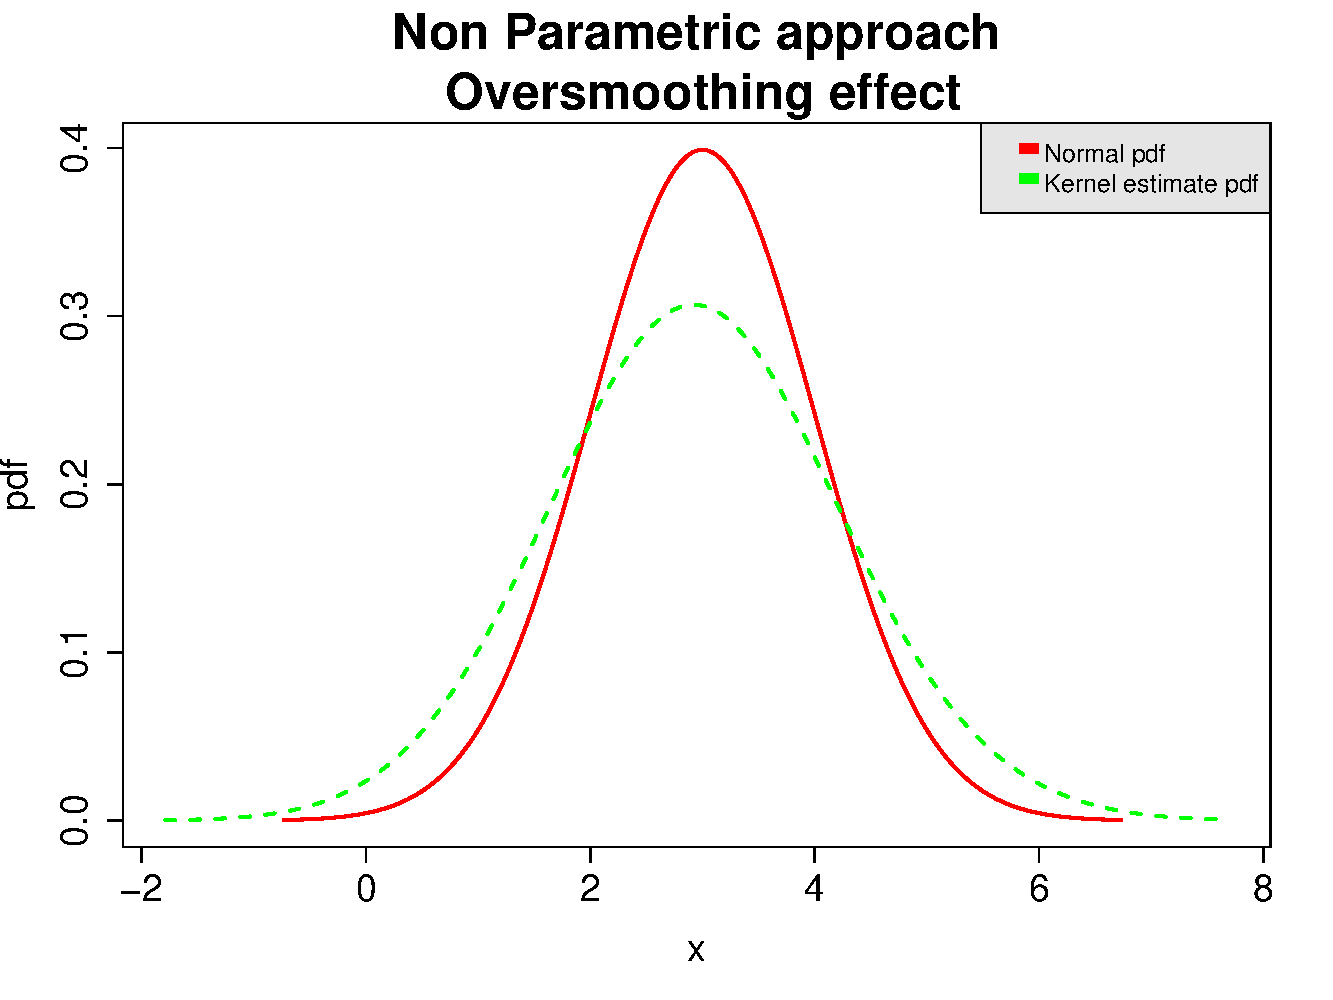
\includegraphics[width=0.50\textwidth]{oversmoothing.pdf}
  \end{center}

  \textbf{\textit{Undersmoothing effect}}\\
  In this case, $h$ is smaller than the optimal choice $h_{opt}$. The effect of the values is more locally focused on the values obtained in the data set than in the optimal case.

  \begin{center}
    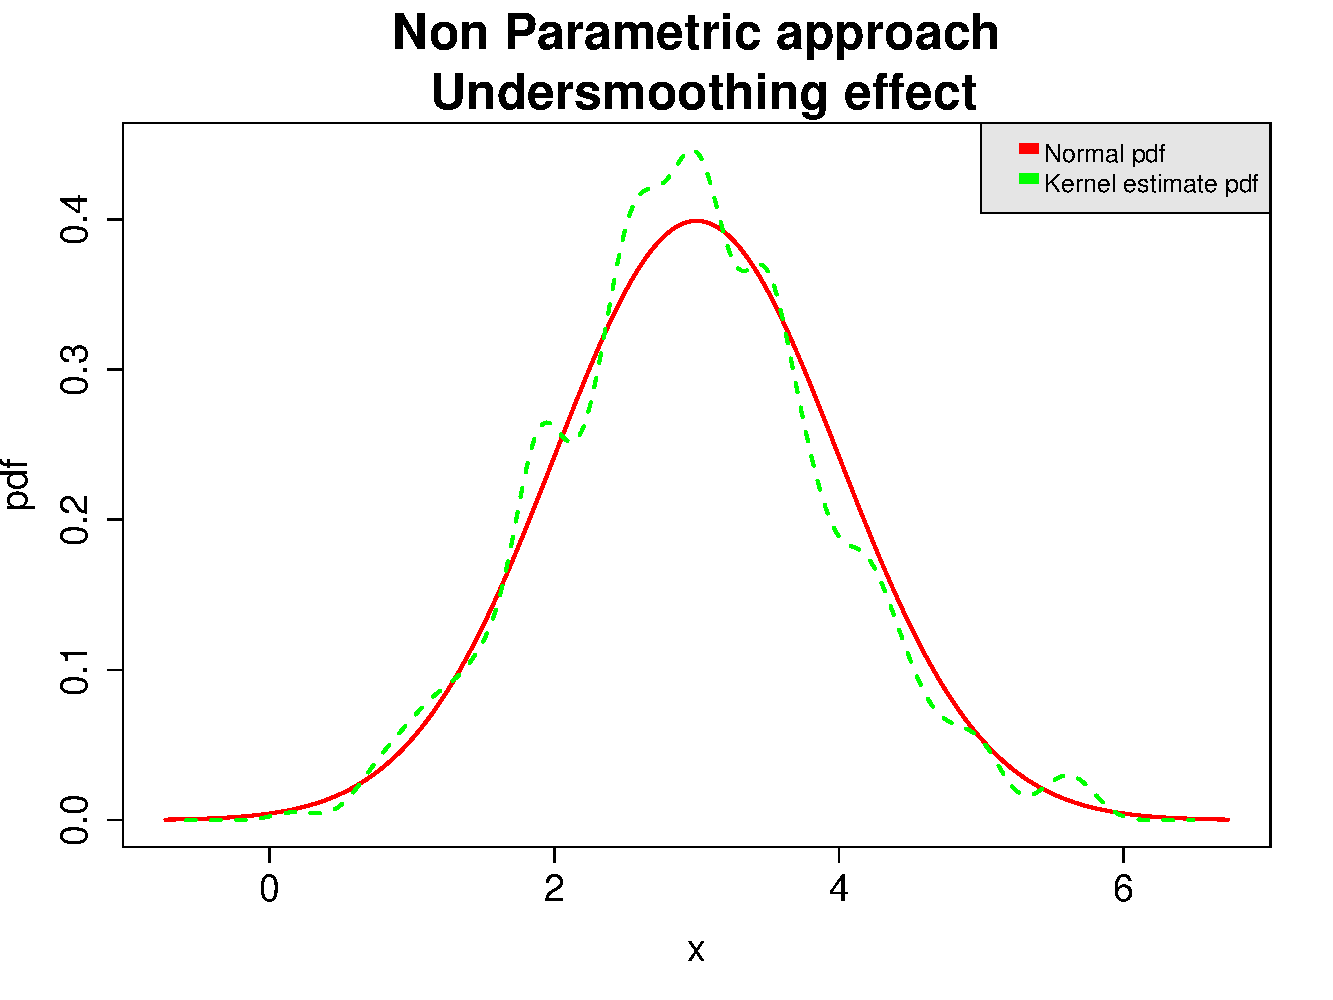
\includegraphics[width=0.60\textwidth]{undersmoothing.pdf}
  \end{center}

  \textbf{\textit{Optimal smoothing}}\\
  Following the previous Silverman rule, for a Gaussian distribution.

  \begin{center}
    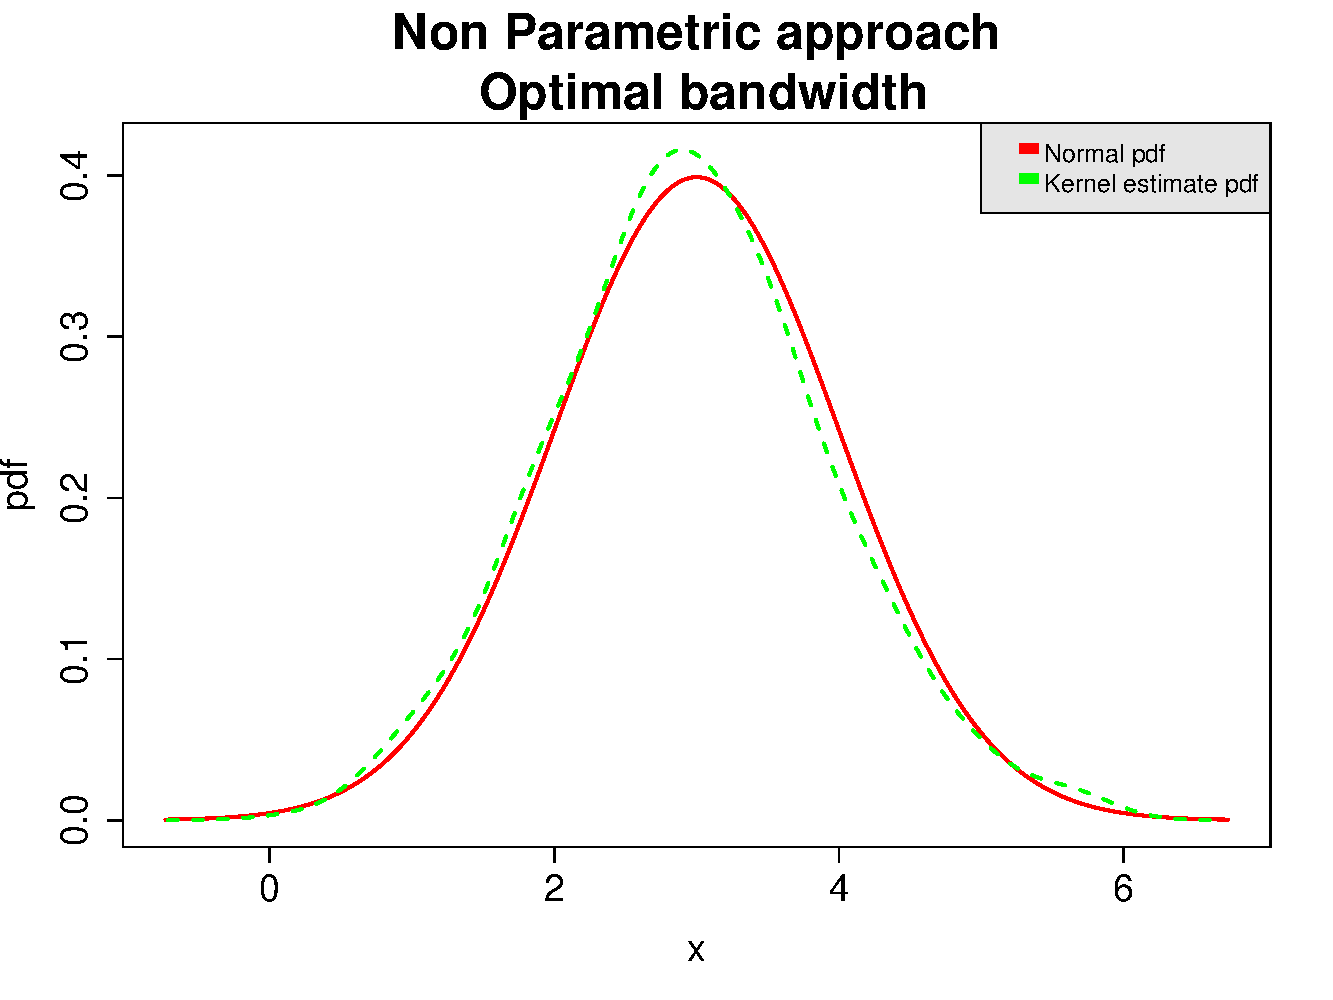
\includegraphics[width=0.50\textwidth]{OKsmoothing.pdf}
  \end{center}


}
